% ----------------------------------------------------------------------------
% DSP
% ----------------------------------------------------------------------------

\chapter{DSP}
\todo{Precisa mudar o nome dos exemplos para exemplo~. Neste caso, a função setup deve ser renomeada para "tilde\_setup")}

Enfim chegamos no processamento de áudio propriamente dito. Digital Signal Processing ou processamento de sinal digital. O PD tem inlets especiais para o processamento de sinal. É fácil reconhecer. Eles são pintados de preto.
\begin{figure}[h!]
	\centering
	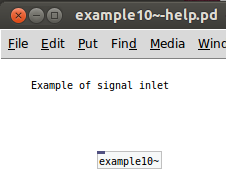
\includegraphics[width=0.7\textwidth]{example10}
	\caption{Primeiro Inlet DSP}
\end{figure}

\section{Primeiro inlet para DSP}
Para trabalharmos com DSP no Pure Data é necessário alguns cuidados. (Veja o
exemplo10) Primeiramente, temos de ter na estrutura de dados um atributo do
tipo t\_float para armazenar o valor de entrada do inlet.

\begin{lstlisting}
typedef struct _example10 {
    t_object x_obj;
    t_float x_f;
/* place to hold inlet's value if it's set by message */
} t_example10;
\end{lstlisting}

Caso trabalhemos com apenas um inlet de DSP, o mesmo pode utilizar o atributo
"mágico" do primeiro inlet da esquerda. Isto pode ser feito com a atribuição do
atributo ao inlet DSP no método setup(). Para isto temos de utilizar o tipo de
classe padrão do Pure Data (CLASS\_DEFAULT). Também é necessário definirmos
qual será o método chamado quando o DSP é iniciado. Este método é adicionado
como os métodos dos inlets vistos anteriormente tendo porém sua mensagem
associada ao tipo "dsp".

\begin{lstlisting}
void example10_setup(void) {
    example10_class = class_new(gensym("example10"),
            (t_newmethod) example10_new, // Constructor
            (t_method) example10_destroy, // Destructor
            sizeof (t_example10),
	    CLASS_DEFAULT,
	    A_GIMME, // Allows various parameters
            0); // LAST argument is ALWAYS zero

  /* this is magic to declare that the leftmost, "main" inlet
     takes signals; other signal inlets are done differently...*/
     CLASS_MAINSIGNALIN(example10_class, t_example10, x_f);

   // This method will add a signal inlet and associate a method to do this
    class_addmethod(example10_class, (t_method) example10_dsp, 
	gensym("dsp"), 0); 

}
\end{lstlisting}
 
A declaração de outros inlets DSP será vista logo adiante.

O próximo passo é definirmos o método DSP definido no setup().

\begin{lstlisting}
static void example10_dsp(t_example10 *x, t_signal **sp){
  dsp_add(example10_perform, 3, sp[0]->s_vec, sp[0]->s_n, x); 
}
\end{lstlisting}

O método associado ao DSP será chamado TODA VEZ QUE O DSP FOR INICIADO. Por
isto, cuidado com alocações de memória, inicialização de variáveis e estas
coisas. Neste método definiremos quem será chamado em cada laço de execução de
processamento de áudio do PD. Neste cado é a função example10\_perform. Este
método recebe o array de sinal que a conexão deste inlet traz. Este sinal está
na variável **sp. Na atribuição acima, passamos para o método perform os
atributos:

\begin{itemize}
\item método perform
\item quantidade de atributos do método
\item vetor de saída
\item tamanho do vetor (tamanho do bloco)
\item instância do nosso external
\end{itemize}

Podemos passar para o método perform quaisquer parâmetros em qualquer ordem. Só
é importante e óbvio que devemos lembrar quais parâmetros foram passados e em
qual ordem. O próximo passo é criar o método perform propriamente dito.

\begin{lstlisting}
static t_int * example10_perform(t_int *w){
   t_float *in = (t_float *)(w[1]);
   int n = (int)(w[2]);
   t_example10 *x = (t_example10 *)(w[3]);

  //(... DO SOMETHING)

  return (w + 4); // proximo bloco
}
\end{lstlisting}

\todo{O que raios há na posição w[0]?}

O método perform receberá como parâmetro um array com os dados que definimos no
método anterior. Neste caso na posição 0 algo que eu não sei o que é, na
posição 1 o vetor de saída, na posição 2 o tamanho do vetor de saída e na
posição 3 a nossa estrutura de dados. Este método deve retornar a próxima
posição do vetor, ou seja, o atributo de entrada + quantidade de atributos do
método + 1.

\section{Vários Inlets DSP}
Podemos ter vários inlets de DSP no nosso external (Veja o exemplo 11). A
criação de inlets adicionais não é feita no método setup() mas sim no
construtor. Só será necessário criar o primeiro inlet se a classe não for do
tipo CLASS\_DEFAULT.

\begin{lstlisting}
// Constructos of the class
void * example11_new(t_symbol *s, int argc, t_atom * argv) {
    t_example11 *x = (t_example11 *) pd_new(example11_class);
    inlet_new(&x->x_obj, &x->x_obj.ob_pd, &s_signal, &s_signal); // second
    inlet_new(&x->x_obj, &x->x_obj.ob_pd, &s_signal, &s_signal); // third
    inlet_new(&x->x_obj, &x->x_obj.ob_pd, &s_signal, &s_signal); // fourth
    return (void *) x;
}
\end{lstlisting}

Nosso método class\_addmethod é exatamente igual ao anterior mas temos uma
mudança na quantidade de parâmetros por causa da quantidade de inlets.

\begin{lstlisting}
static void example11_dsp(t_example11 *x, t_signal **sp){
  dsp_add(example11_perform, 6, sp[0]->s_vec, sp[0]->s_n, x);
}
\end{lstlisting}

Note que precisamos agora alterar a quantidade de parâmetros passadas ao método
perform. O método perform ficará assim:
\begin{lstlisting}
static t_int * example11_perform(t_int *w){
   t_float *in1 = (t_float *)(w[1]);
   t_float *in2 = (t_float *)(w[2]);
   t_float *in3 = (t_float *)(w[3]);
   t_float *in4 = (t_float *)(w[4]);
   int n = (int)(w[5]);
   t_example11 *x = (t_example11 *)(w[6]);
   // DO SOMETHING...
  return (w + 7); // proximo bloco
}
\end{lstlisting}

Nosso external pronto deverá ter a seguinte aparência:
\begin{figure}[h!]
	\centering
	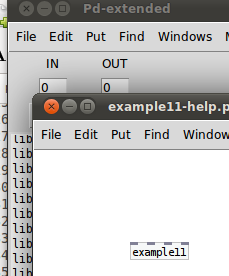
\includegraphics[width=0.7\textwidth]{example11}
	\caption{Vários inlets DSP.}
\end{figure}

\section{Primeiro outlet DSP}

A criação dos outlets é feita no construtor do external (Veja o exemplo12) e
não é necessário termos adicionado os outlets a estrutura da classe.

\begin{lstlisting}
// Constructos of the class
void * example12_new(t_symbol *s, int argc, t_atom * argv) {
    t_example12 *x = (t_example12 *) pd_new(example12_class);
    outlet_new(&x->x_obj, &s_signal); // first signal outlet
    outlet_new(&x->x_obj, &s_signal); // second signal outlet
    outlet_new(&x->x_obj, &s_signal); // third signal outlet
    outlet_new(&x->x_obj, &s_signal); // fourth signal outlet
    return (void *) x;
}
\end{lstlisting}

Sabendo que temos 4 outlets, a definição do nosso método perform será idêntica
ao da criação de 4 inlets.

\begin{lstlisting}
static void example12_dsp(t_example12 *x, t_signal **sp){
  dsp_add(example12_perform, 6, sp[0]->s_vec, sp[0]->s_n, x);
}
\end{lstlisting}

O método perform também será idêntico ao do exemplo com 4 inlets, porém o mesmo
receberá 4 outlets.

\begin{lstlisting}
static t_int * example12_perform(t_int *w){
   t_float *out1 = (t_float *)(w[1]);
   t_float *out2 = (t_float *)(w[2]);
   t_float *out3 = (t_float *)(w[3]);
   t_float *out4 = (t_float *)(w[4]);
   int n = (int)(w[5]);
   t_example12 *x = (t_example12 *)(w[6]);
  // DO SOMETHING
  return (w + 7); // proximo bloco
}
\end{lstlisting}

\begin{figure}[h!]
	\centering
	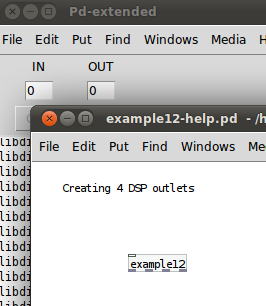
\includegraphics[width=0.7\textwidth]{example12}
	\caption{Primeiro Outlet DSP.}
\end{figure}

\section{Inlets e outlets DSP}
Nosso próximo exemplo (Veja o exemplo 13) mistura no mesmo objeto inlets e
outlets DSP. Uma coisa bastante comum. Acredito que seja óbvio a construção do
mesmo. Não precisamos associar estes inlets e outlets a nossa estrutura de
dados. Precisamos apenas criar os inlets e outlets no construtor (lembre-se que
o primeiro inlet já foi criado no método setup. Ele é mágico!).

\begin{lstlisting}
static t_int * example13_perform(t_int *w){
   t_float *in1 = (t_float *)(w[1]);
   t_float *in2 = (t_float *)(w[2]);
   t_float *in3 = (t_float *)(w[3]);
   t_float *in4 = (t_float *)(w[4]);
   t_float *out1 = (t_float *)(w[5]);
   t_float *out2 = (t_float *)(w[6]);
   t_float *out3 = (t_float *)(w[7]);
   t_float *out4 = (t_float *)(w[8]);
   int n = (int)(w[9]);
   t_example13 *x = (t_example13 *)(w[10]);
  return (w + 11); // proximo bloco
}
\end{lstlisting}

No método seguinte avisamos o método perform do tamanho dos dados.
\begin{lstlisting}
static void example13_dsp(t_example13 *x, t_signal **sp){
  dsp_add(example13_perform, 10, sp[0]->s_vec, sp[0]->s_n, x);
}
\end{lstlisting}

No método perform teremos primeiro os buffers de entrada e depois os buffers de
saída.

\begin{lstlisting}
static t_int * example13_perform(t_int *w){
   t_float *in1 = (t_float *)(w[1]);
   t_float *in2 = (t_float *)(w[2]);
   t_float *in3 = (t_float *)(w[3]);
   t_float *in4 = (t_float *)(w[4]);
   t_float *out1 = (t_float *)(w[5]);
   t_float *out2 = (t_float *)(w[6]);
   t_float *out3 = (t_float *)(w[7]);
   t_float *out4 = (t_float *)(w[8]);
   int n = (int)(w[9]);
   t_example13 *x = (t_example13 *)(w[10]);
   //DO IT!
  return (w + 11); // proximo bloco
}
\end{lstlisting}

\begin{figure}[h!]
	\centering
	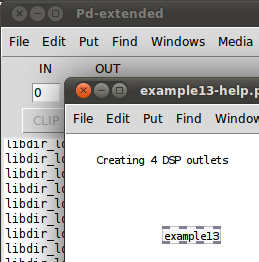
\includegraphics[width=0.7\textwidth]{example13}
	\caption{Vários inlets e outlets DSP.}
\end{figure}

\section{Inlets e outlets DSP criados dinamicamente}

Podemos definir um parâmetro no construtor que nos diga a quantidade de inlets
e/ou de outlets DSP que um external terá. Neste caso, temos algumas
possibilidades. A primeira é passarmos para o construtor a informação de quantos inlets e
outlets teremos na função dsp (veja o exemplo 17) e armazenarmos na nossa estrutura de dados.

\begin{lstlisting}
typedef struct _example17 {
    t_object x_obj;
    t_int outlet_counter;
    t_int inlet_counter;
} t_example17;

void * example17_new(t_symbol *s, t_int inlet_counter, t_int outlet_counter) {
    t_example17 *x = (t_example17 *) pd_new(example17_class);

    post("inlet counter %d",inlet_counter);
    post("outlet counter %d",outlet_counter);

    x->inlet_counter = inlet_counter;
    x->outlet_counter = outlet_counter;

    int i;
    // Let's create the inlets and outlets
    for(i = 0 ; i < inlet_counter ; i++)
	inlet_new(&x->x_obj, &x->x_obj.ob_pd, &s_signal, &s_signal);

    for(i = 0 ; i < outlet_counter ; i++)
	outlet_new(&x->x_obj, &s_signal);

    return (void *) x;
}
\end{lstlisting}

Na passagem de parâmetro para o DSP usamos estas variáveis para contar quantos parâmetros serão usados.

\begin{lstlisting}
static t_int * example17_perform(t_int *w){
   t_example17 *x = (t_example17 *)(w[1]);
   int n = (int)(w[2]);

   int i;
   for(i = 0 ; i < x->inlet_counter ; i++){
	// DO something with the input
	}

   for(i = 0 ; i < x->outlet_counter ; i++){
	// DO something with the output
	}

  return (w + 2 + x->inlet_counter + x->outlet_counter + 1);
}

static void example17_dsp(t_example17 *x, t_signal **sp){
  int qtd = x->inlet_counter + x->outlet_counter + 2;
  dsp_add(example17_perform, qtd , x, sp[0]->s_n, sp[0]->s_vec);
}
\end{lstlisting}


A segunda é usar outro método que baseia-se no modelo de alocação de memória do pd. Criamos um vetor e 
apontamos este vetor para o dado da entrada / saída do external. Assim podemos utilizar a estrutura
amarrada ao external para produzir / consumir o dado. Veja o exemplo 19.

\begin{lstlisting}
void example19_setup(void) {
    example19_class = class_new(gensym("example19"),
            (t_newmethod) example19_new, // Constructor
            (t_method) example19_destroy, // Destructor
            sizeof (t_example19),
	    CLASS_NOINLET,
	    A_DEFFLOAT, // # of inlets
            0); // LAST argument is ALWAYS zero

    class_addmethod(example19_class, (t_method) example19_dsp, gensym("dsp"), 0);
}
\end{lstlisting}

Neste ponto, esta solução é bastante parecida com a anterior e poderia ser usada também com uma quantidade
variável de outlets. A alteração está na estrutura da classe.

\begin{lstlisting}
typedef struct _example19 {
    t_object x_obj;
    t_sample * outvec[64]; // 64 is a magic number!
    t_int inlet_counter;
} t_example19;
\end{lstlisting}

Ok. 64 não é um número mágico. Ele é o tamanho de bloco padrão do Pd. Para que esta solução
seja genérica o suficiente é melhor usar a função sys\_getblksize() para verificarmos o tamanho
do bloco e alocarmos isto corretamente. Deste jeito isto pode dar estouro de ponteiro. 

\begin{lstlisting}
void * example19_new(t_symbol *s, t_floatarg inlet_counter, t_floatarg outlet_counter) {
    t_example19 *x = (t_example19 *) pd_new(example19_class);

    post("inlet counter %f", inlet_counter);

    x->inlet_counter = inlet_counter;

    int i;
    for(i = 0 ; i < inlet_counter ; i++)
	inlet_new(&x->x_obj, &x->x_obj.ob_pd, &s_signal, &s_signal);

    return (void *) x;
}
\end{lstlisting}

O construtor continua criando a quantidade de outlets que precisamos. Neste ponto poderia
ser utilizado a função malloc para alocar o vetor com os dados de maneira inteligente em 
vez de usar o 64 mágico.

\begin{lstlisting}
static void example19_dsp(t_example19 *x, t_signal **sp){
    short i;
    for (i = 0; i < x->inlet_counter; i++)
        x->outvec[i] = sp[i]->s_vec; // Put the inlets data into my structure
  dsp_add(example19_perform, 1 , x);
}
\end{lstlisting}

O método DSP não fará mais que passar o próprio objeto ao método perform. Poderia não passar nem o objeto.

\begin{lstlisting}
static t_int * example19_perform(t_int *w){
   t_example19 *x = (t_example19 *)(w[1]);
   // Call DSP function or start DSP thread
  return (w + 2);
}
\end{lstlisting}

A função perform não precisa necessariamente fazer mais do que despertar o processo consumidor e
liberar o processamento no Pd. E este é um ponto que considero importante para levantar outro questionamento.

O Pd precisa que os blocos terminem em determinado tempo. Qual seria este tempo? Imaginemos que o bloco seja de 
64 amostras. Se tivermos uma amostragem de áudio de 44.100 amostras por segundo precisamos que o bloco encerre seu 
processamento em um pouco mais de 1 milisegundo. Parece rápido mas seu computador é mais rápido que isto.
Criar um processo consumidor e fazê-lo liberando o bloco de processamento
pode ser uma abordagem melhor para processos baseados em fluxo, como escrita em arquivos. Para isto precisamos utilizar outra
função em outra thread e este é nosso próximo assunto.

\todo{Vale a pena mostrar como fazer o loop entre as amostras ou é óbvio?}
